\documentclass[a4paper,12pt]{article}
\usepackage[utf8]{inputenc}
\usepackage[ngerman]{babel}
\usepackage{amsmath}
\usepackage{amssymb}
\usepackage{amsthm}
\usepackage{geometry}
\usepackage{graphicx}
\usepackage[hidelinks]{hyperref}
\usepackage{listings}
\usepackage{xcolor}
\usepackage{enumitem}
\usepackage{microtype}

\geometry{margin=2.5cm}

\theoremstyle{definition}
\newtheorem{definition}{Definition}
\newtheorem{beispiel}{Beispiel}
\newtheorem{satz}{Satz}
\newtheorem{lemma}{Lemma}
\newtheorem{bemerkung}{Bemerkung}
\newtheorem{annahme}{Annahme}

\setlist[itemize,1]{label=--}

% ---------- Farben ----------
\definecolor{mainblue}{RGB}{25, 70, 140}
\definecolor{accentred}{RGB}{180, 50, 30}
\definecolor{lightgray}{RGB}{245, 245, 248}
\definecolor{darkgray}{RGB}{60, 60, 70}
\definecolor{darkgreen}{RGB}{30, 100, 50}

\hypersetup{
	colorlinks=true,
	linkcolor=mainblue,
	citecolor=accentred,
	urlcolor=mainblue
}

\lstset{
	basicstyle=\ttfamily\small,
	keywordstyle=\color{blue},
	commentstyle=\color{gray},
	stringstyle=\color{red},
	numbers=left,
	numberstyle=\tiny,
	breaklines=true,
	frame=single,
	literate=%
	{Ö}{{\"O}}1
	{Ä}{{\"A}}1
	{Ü}{{\"U}}1
	{ß}{{\ss}}1
	{ü}{{\"u}}1
	{ä}{{\"a}}1
	{ö}{{\"o}}1
	{Σ}{{$\Sigma$}}1
	{→}{{$\rightarrow$}}1
	{⊆}{{$\subseteq$}}1
	{⊇}{{$\supseteq$}}1
	{≥}{{$\geq$}}1
}

\title{Optimierungsmodelle für Windenergieanlagen:\\
Nabenhöhe, Rotorblattlänge, Blattanzahl\\
und Dimensionierung von Windradfamilien}
\author{Stephan Epp}
\date{13. Juni 2026}

\begin{document}

\maketitle

\tableofcontents
\newpage

\section{Einführung}

Die wirtschaftliche und technische Auslegung einer Windenergieanlage (WEA) ist ein mehrdimensionales Optimierungsproblem, bei dem mehrere konstruktive Freiheitsgrade -- die Nabenhöhe $h$, die Rotorblattlänge $r$, die Blattanzahl $B$ sowie die Anzahl $N$ gleichartiger Anlagen innerhalb einer Windradfamilie (Windpark) -- in einem nichttrivialen Zusammenspiel mit physikalischen Ertragsmodellen und ökonomischen Kostenmodellen stehen. Jede dieser Größen erhöht für sich genommen den potenziellen Energieertrag, ist jedoch mit überproportional wachsenden Kosten, Materialbelastungen oder aerodynamischen Verlusten verbunden. Daraus resultiert in jedem Fall ein inneres Optimum, das sich formal als Maximierungsproblem einer Nettowertfunktion
\[
N(\cdot) = E(\cdot) - K(\cdot)
\]
beschreiben lässt, wobei $E$ den über die Lebensdauer diskontierten Energieertrag und $K$ die zugehörigen Investitions- bzw. Grenzkosten bezeichnet.

\subsection{Problemstellung}

Gegeben seien:
\begin{itemize}
	\item ein Höhenprofil der Windgeschwindigkeit $v(h)$,
	\item ein aerodynamisches Leistungsmodell $P(r, B, v)$ basierend auf der Betz'schen Theorie,
	\item Kostenfunktionen $K_h(h)$, $K_r(r)$ für Turm bzw. Rotorblätter, die aus Skalierungsgesetzen der Materialwissenschaft folgen,
	\item ein Nachlaufmodell (Wake-Modell) nach Jensen für die gegenseitige Beeinflussung von $N$ Anlagen in einer Windradfamilie.
\end{itemize}

\textbf{Ziel:} Bestimme für einen gegebenen Standorttyp (Onshore/Land oder Offshore/Meer) die Parameterkombination $(h^*, r^*, B^*, N^*)$, die den Gesamtnettowert über die Lebensdauer $T$ maximiert.

\subsection{Motivation}

Anders als beim Subgraph Algorithmus, bei dem eine kombinatorische Struktur (Graphenvergleich) im Zentrum steht, handelt es sich hier um eine Familie kontinuierlicher und diskreter Optimierungsprobleme mit jeweils einem dominanten Ertragsterm (monoton wachsend, sublinear in den hohen Potenzen) und einem dominanten Kostenterm (monoton wachsend, mit höherer Potenz oder höherem Skalierungsexponenten). Das gemeinsame methodische Prinzip -- die Bestimmung eines Schnittpunktes zweier gegenläufiger Skalierungsgesetze -- erlaubt eine einheitliche formale Behandlung aller vier Teilprobleme nach demselben Schema: Aufstellung von $E(\cdot)$ und $K(\cdot)$, Bildung von $N(\cdot) = E(\cdot)-K(\cdot)$, Nullsetzen der Ableitung und Verifikation über die zweite Ableitung (bzw. diskrete Differenzenanalyse für $B$ und $N$).

\section{Grundlagen}

\subsection{Definitionen}

\begin{definition}[Hellmann-Potenzgesetz]
\label{def:hellmann}
Die Windgeschwindigkeit $v(h)$ in Höhe $h$ über einer Referenzhöhe $h_{\mathrm{ref}}$ mit Referenzgeschwindigkeit $v_{\mathrm{ref}}$ ist gegeben durch
\[
v(h) = v_{\mathrm{ref}} \left(\frac{h}{h_{\mathrm{ref}}}\right)^{\alpha},
\]
wobei $\alpha$ der Hellmann-Exponent (Rauigkeitsexponent) ist. Typische Werte sind $\alpha \approx 0{,}10$ für glatte Wasserflächen (Offshore), $\alpha \approx 0{,}14$ für offenes Ackerland (Onshore) und $\alpha \approx 0{,}25$ für bewaldetes oder städtisches Gelände.
\end{definition}

\begin{definition}[Betz'sches Leistungsgesetz]
\label{def:betz}
Die einer Luftströmung mit Geschwindigkeit $v$ durch eine Rotorfläche $A = \pi r^2$ entnehmbare Leistung ist
\[
P(r, v) = \tfrac{1}{2}\,\rho\, A\, C_p\, v^3 = \tfrac{1}{2}\,\rho\, \pi r^2\, C_p\, v^3,
\]
wobei $\rho$ die Luftdichte und $C_p \le C_{p,\max} = \tfrac{16}{27} \approx 0{,}593$ (Betz-Limit) der Leistungsbeiwert ist.
\end{definition}

\begin{definition}[Kapazitätsfaktor]
\label{def:cf}
Der Kapazitätsfaktor $c_f \in (0,1)$ beschreibt das Verhältnis der tatsächlich über ein Jahr erzeugten Energie zur theoretischen Energie bei durchgehendem Volllastbetrieb. Für moderne Anlagen liegt $c_f$ typischerweise zwischen $0{,}25$ (Land) und $0{,}45$ (Meer).
\end{definition}

\begin{definition}[Jensen-Nachlaufmodell]
\label{def:jensen}
Im linearen Nachlaufmodell nach Jensen (1983) reduziert sich die Windgeschwindigkeit hinter einer Turbine mit Schubbeiwert $C_T$ im Abstand $s = m \cdot D$ (mit Rotordurchmesser $D$) auf
\[
v_{\mathrm{wake}} = v_0 \left[1 - \frac{1-\sqrt{1-C_T}}{(1 + 2 k_w m)^2}\right],
\]
wobei $k_w$ der Nachlauf-Expansionskoeffizient ist ($k_w \approx 0{,}075$ Onshore, $k_w \approx 0{,}04$ Offshore).
\end{definition}

\begin{annahme}[Lebensdauer und Diskontierung]
\label{ann:lebensdauer}
Die wirtschaftliche Lebensdauer einer WEA wird mit $T = 20$ Jahren angenommen, bei $8760$ Betriebsstunden pro Jahr und einem mittleren Strompreis $p$ (EUR/kWh), der über die Lebensdauer als konstant angenommen wird (vereinfachte, undiskontierte Betrachtung zur Wahrung der Übersichtlichkeit der formalen Aussagen).
\end{annahme}

\section{Optimierung der Nabenhöhe}

\subsection{Modellbildung}

Aus Definition~\ref{def:hellmann} und Definition~\ref{def:betz} folgt für die Leistung in Abhängigkeit der Nabenhöhe bei festem Rotorradius $r$:
\[
P(h) = \tfrac{1}{2}\,\rho\, \pi r^2\, C_p\, v_{\mathrm{ref}}^3 \left(\frac{h}{h_{\mathrm{ref}}}\right)^{3\alpha}.
\]
Der über die Lebensdauer erzielte Ertrag (Annahme~\ref{ann:lebensdauer}) ist
\[
E(h) = P(h) \cdot 8760 \cdot c_f \cdot T \cdot p = \kappa_E \cdot h^{3\alpha}, \qquad \kappa_E := \tfrac{1}{2}\rho \pi r^2 C_p \left(\frac{v_{\mathrm{ref}}}{h_{\mathrm{ref}}^{\alpha}}\right)^3 \cdot 8760\, c_f\, T\, p.
\]

\begin{satz}[Strikte Konkavität des Ertragsterms in $h$]
\label{satz:konkav_ertrag}
Für $\alpha \in (0,1)$ und $h>0$ ist $E(h) = \kappa_E h^{3\alpha}$ streng konkav, sofern $3\alpha < 1$, und streng konvex für $3\alpha>1$. Für $\alpha \approx 0{,}10$ bis $0{,}25$ gilt $3\alpha \in (0{,}3, 0{,}75) \subset (0,1)$, also ist $E(h)$ in den praktisch relevanten Fällen streng konkav.
\end{satz}

\begin{proof}
Es gilt $E'(h) = 3\alpha \kappa_E h^{3\alpha-1}$ und $E''(h) = 3\alpha(3\alpha-1)\kappa_E h^{3\alpha-2}$. Da $\kappa_E>0$ und $h^{3\alpha-2}>0$ für $h>0$, hat $E''(h)$ das Vorzeichen von $(3\alpha-1)$. Für $3\alpha<1$ ist $E''(h)<0$, also $E$ streng konkav. \qedhere
\end{proof}

Für die Materialkosten des Turms wird ein Skalierungsgesetz mit Exponent $\beta>1$ angesetzt, das die mit der Höhe überproportional zunehmenden Anforderungen an Knickstabilität, Wandstärke, Fundament und Transport/Montage abbildet:
\[
K(h) = \kappa_K \cdot h^{\beta}, \qquad \beta > 3\alpha.
\]

\begin{lemma}[Existenz und Eindeutigkeit des Höhenoptimums]
\label{lem:hoehe_existenz}
Sei $N(h) = E(h) - K(h) = \kappa_E h^{3\alpha} - \kappa_K h^{\beta}$ mit $\kappa_E,\kappa_K>0$ und $\beta > 3\alpha > 0$. Dann besitzt $N(h)$ für $h>0$ genau ein lokales Maximum, und dieses ist global.
\end{lemma}

\begin{proof}
Es gilt
\[
N'(h) = 3\alpha\,\kappa_E\, h^{3\alpha-1} - \beta\,\kappa_K\, h^{\beta-1}.
\]
Da $\beta>3\alpha$, ist $h^{\beta-1}/h^{3\alpha-1} = h^{\beta-3\alpha}$ streng monoton wachsend in $h$ (für $h>0$, da $\beta-3\alpha>0$) und nimmt Werte in $(0,\infty)$ an. Setze $N'(h)=0$:
\[
3\alpha\,\kappa_E\, h^{3\alpha-1} = \beta\,\kappa_K\, h^{\beta-1}
\quad\Longleftrightarrow\quad
h^{\beta-3\alpha} = \frac{3\alpha\,\kappa_E}{\beta\,\kappa_K}.
\]
Da die rechte Seite eine positive Konstante ist und $h \mapsto h^{\beta-3\alpha}$ für $h>0$ eine Bijektion auf $(0,\infty)$ ist (streng monoton wachsend, stetig, $\lim_{h\to0^+}=0$, $\lim_{h\to\infty}=\infty$), existiert genau eine Lösung
\[
h^* = \left(\frac{3\alpha\,\kappa_E}{\beta\,\kappa_K}\right)^{\frac{1}{\beta-3\alpha}}.
\]
Für $h<h^*$ ist $N'(h)>0$ (da $h^{\beta-3\alpha} < $ rechte Seite, also $3\alpha\kappa_E h^{3\alpha-1} > \beta\kappa_K h^{\beta-1}$), für $h>h^*$ ist $N'(h)<0$. Damit ist $h^*$ ein striktes globales Maximum auf $(0,\infty)$. \qedhere
\end{proof}

\begin{satz}[Optimale Nabenhöhe]
\label{satz:hoehe_optimal}
Die optimale Nabenhöhe ist
\[
h^* = \left(\frac{3\alpha\,\kappa_E}{\beta\,\kappa_K}\right)^{\frac{1}{\beta-3\alpha}}
\]
mit $\kappa_E$ und $\kappa_K$ wie oben definiert. Sie ist streng monoton wachsend in $\alpha$ (für festes $\beta$): Standorte mit höherem Rauigkeitsexponenten (Land, $\alpha\approx0{,}14$) profitieren stärker von größerer Höhe als Standorte mit niedrigem $\alpha$ (Meer, $\alpha\approx0{,}10$), relativ zu identischen Kostenparametern.
\end{satz}

\begin{proof}
Folgt direkt aus Lemma~\ref{lem:hoehe_existenz}. Für die Monotonie in $\alpha$ betrachte
\[
\ln h^* = \frac{1}{\beta-3\alpha}\left(\ln(3\alpha) + \ln\kappa_E - \ln\beta - \ln\kappa_K\right).
\]
Die partielle Ableitung nach $\alpha$ besteht aus zwei positiven Anteilen: (i) der Term $\frac{1}{\beta-3\alpha}$ wächst mit $\alpha$ (Nenner wird kleiner), (ii) $\ln(3\alpha)$ wächst mit $\alpha$. Beide Effekte sind für $\alpha \in (0, \beta/3)$ positiv, sodass $\frac{\partial h^*}{\partial \alpha}>0$. \qedhere
\end{proof}

\begin{satz}[Skalierungselastizität der optimalen Höhe]
\label{satz:elastizitaet_hoehe}
Sei $h^*(\kappa_E,\kappa_K)$ die optimale Höhe aus Satz~\ref{satz:hoehe_optimal}, aufgefasst als Funktion der Ertrags- bzw. Kostenkonstanten bei festen Exponenten $\alpha,\beta$. Dann gelten die Elastizitäten
\[
\frac{\partial \ln h^*}{\partial \ln \kappa_E} = \frac{1}{\beta-3\alpha} > 0,
\qquad
\frac{\partial \ln h^*}{\partial \ln \kappa_K} = -\frac{1}{\beta-3\alpha} < 0.
\]
Insbesondere bewirkt eine relative Erhöhung der Ertragskonstante $\kappa_E$ um $x\%$ stets eine \emph{geringere} relative Erhöhung von $h^*$ (da $\beta-3\alpha>1$ in den hier betrachteten Parameterregimen, also $\frac{1}{\beta-3\alpha}<1$), während dieselbe relative Senkung der Kostenkonstante $\kappa_K$ um $x\%$ eine betragsmäßig identische, aber gegenläufige Wirkung auf $h^*$ hat.
\end{satz}

\begin{proof}
Aus Satz~\ref{satz:hoehe_optimal} folgt
\[
\ln h^* = \frac{1}{\beta-3\alpha}\Bigl(\ln(3\alpha) - \ln\beta + \ln\kappa_E - \ln\kappa_K\Bigr).
\]
Differentiation nach $\ln\kappa_E$ bei festem $\alpha,\beta,\kappa_K$ liefert unmittelbar $\frac{\partial \ln h^*}{\partial\ln\kappa_E} = \frac{1}{\beta-3\alpha}$, da alle übrigen Terme der Klammer nicht von $\kappa_E$ abhängen und $\frac{\partial}{\partial\ln\kappa_E}\ln\kappa_E=1$. Analog folgt $\frac{\partial \ln h^*}{\partial\ln\kappa_K} = -\frac{1}{\beta-3\alpha}$, da $\ln\kappa_K$ mit negativem Vorzeichen in der Klammer steht. Für $\alpha=0{,}14$ und $\beta=2{,}6$ ist $\beta-3\alpha=2{,}6-0{,}42=2{,}18>1$, also $\frac{1}{\beta-3\alpha}\approx0{,}459<1$, was die behauptete Dämpfung zeigt. \qedhere
\end{proof}

\begin{bemerkung}
Satz~\ref{satz:elastizitaet_hoehe} hat eine unmittelbare praktische Konsequenz: Technologische Fortschritte, die den Ertragsfaktor $\kappa_E$ erhöhen (z.\,B. verbesserter $C_p$ durch aerodynamische Optimierung der Blätter, siehe Abschnitt~5), wirken sich nur gedämpft (Elastizität $\approx0{,}46$) auf die ökonomisch optimale Nabenhöhe aus -- eine Verdopplung von $\kappa_E$ erhöht $h^*$ nur um den Faktor $2^{0{,}459}\approx1{,}37$, also um etwa $37\%$. Umgekehrt führt eine Halbierung der Turmkosten $\kappa_K$ (z.\,B. durch neue Materialien oder Fertigungsverfahren) zu einer Erhöhung von $h^*$ um denselben Faktor $1{,}37$. Diese Symmetrie der Elastizitäten mit entgegengesetztem Vorzeichen ist eine direkte Folge der multiplikativen Struktur von $h^*$ als Quotient der beiden Konstanten.
\end{bemerkung}

\subsection{Numerische Auswertung}

Mit den Parametern $\rho=1{,}225\,\mathrm{kg/m^3}$, $C_p=0{,}45$, $r=93{,}6\,\mathrm{m}$ (Ergebnis aus Abschnitt~\ref{sec:blattlaenge}), $v_{\mathrm{ref}}=6\,\mathrm{m/s}$ bei $h_{\mathrm{ref}}=10\,\mathrm{m}$, $c_f=0{,}35$, $T=20$ Jahre, $p=0{,}07\,\mathrm{EUR/kWh}$ und $\beta=2{,}6$ ergibt sich für $\alpha=0{,}14$ (Onshore) ein Optimum bei
\[
h^* \approx 154\,\mathrm{m}.
\]

\begin{figure}[h]
	\centering
	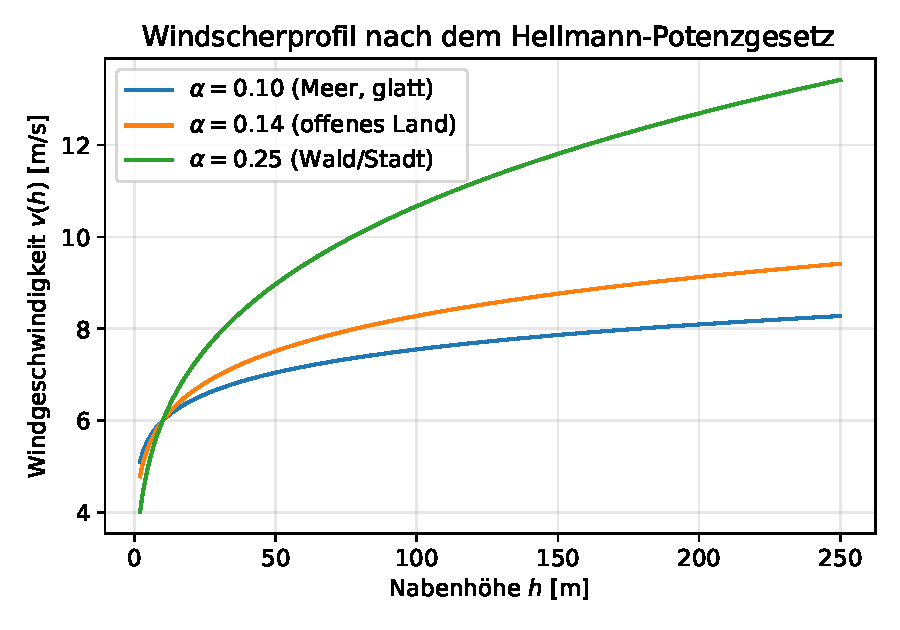
\includegraphics[width=0.85\textwidth]{plots/windprofil.pdf}
	\caption{Windscherprofil $v(h)$ nach dem Hellmann-Potenzgesetz für drei Rauigkeitsklassen. Mit zunehmendem $\alpha$ (rauere Oberfläche) steigt die Windgeschwindigkeit mit der Höhe stärker an, was den Anreiz für höhere Türme erhöht.}
	\label{fig:windprofil}
\end{figure}

\textbf{Beschreibung von Abbildung~\ref{fig:windprofil}.}
Die Abbildung zeigt drei Kurven $v(h) = v_{\mathrm{ref}}(h/h_{\mathrm{ref}})^\alpha$ für $\alpha\in\{0{,}10,\,0{,}14,\,0{,}25\}$ über dem Höhenbereich $h\in[2,250]\,\mathrm{m}$, normiert auf $v_{\mathrm{ref}}=6\,\mathrm{m/s}$ bei $h_{\mathrm{ref}}=10\,\mathrm{m}$. Alle drei Kurven sind konkave, monoton wachsende Potenzfunktionen mit gemeinsamem Startpunkt bei $h_{\mathrm{ref}}$. Die Kurve mit $\alpha=0{,}25$ (Wald/Stadt) verläuft zunächst am flachsten in Bodennähe -- d.\,h. in geringer Höhe ist die Windgeschwindigkeit dort am kleinsten --, überholt aber mit zunehmender Höhe die beiden anderen Kurven, da der Exponent $\alpha$ direkt die Krümmung bzw. Wachstumsrate $v'(h)\propto \alpha h^{\alpha-1}$ bestimmt: Je größer $\alpha$, desto stärker der relative Geschwindigkeitszuwachs pro Höhenmeter (bei gleichbleibend abnehmender absoluter Steigung). Die Kurve mit $\alpha=0{,}10$ (Offshore) ist die flachste über den gesamten Bereich; sie nähert sich für große $h$ einem nahezu horizontalen Verlauf, was bedeutet, dass auf See zusätzliche Nabenhöhe nur einen geringen Geschwindigkeitszuwachs erbringt. Dies ist die physikalische Grundlage für das in Satz~\ref{satz:hoehe_optimal} bewiesene Resultat, dass $h^*$ streng monoton in $\alpha$ wächst: Je steiler das Windprofil mit der Höhe ansteigt (großes $\alpha$), desto stärker rechtfertigt sich ein höherer Turm.

\begin{figure}[h]
	\centering
	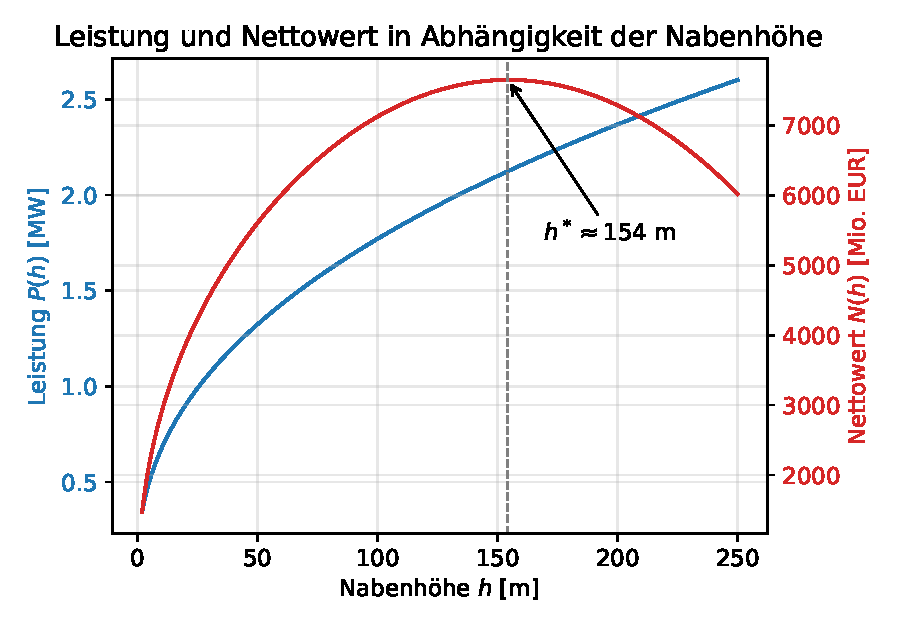
\includegraphics[width=0.85\textwidth]{plots/hoehe_optimierung.pdf}
	\caption{Leistung $P(h)$ (links, blau) und Nettowert $N(h)=E(h)-K(h)$ (rechts, rot) über der Nabenhöhe für $\alpha=0{,}14$. Während $P(h)$ monoton wächst, besitzt $N(h)$ ein eindeutiges inneres Maximum bei $h^*\approx154\,\mathrm{m}$, das aus dem Schnittpunkt des sublinearen Ertragswachstums ($h^{3\alpha}$, $3\alpha=0{,}42$) mit dem superlinearen Kostenwachstum ($h^{2{,}6}$) resultiert.}
	\label{fig:hoehe}
\end{figure}

\textbf{Beschreibung von Abbildung~\ref{fig:hoehe}.}
Die Abbildung verwendet zwei Ordinatenachsen über derselben Abszisse $h\in[2,250]\,\mathrm{m}$. Die linke (blaue) Achse zeigt die reine Rotorleistung $P(h)$ in Megawatt; diese Kurve ist nach Satz~\ref{satz:konkav_ertrag} streng konkav und monoton wachsend, mit abnehmender Steigung $P'(h)\propto h^{3\alpha-1}=h^{-0{,}58}$ -- die Kurve flacht also ab, erreicht aber niemals ein Maximum, da $P(h)\to\infty$ für $h\to\infty$ (wenn auch sehr langsam, da $3\alpha=0{,}42<1$). Die rechte (rote) Achse zeigt den Nettowert $N(h)$ in Millionen Euro über $20$ Betriebsjahre. Diese Kurve startet bei $h\to0$ nahe Null (da sowohl $E(h)\to0$ als auch $K(h)\to0$, aber $E(h)$ dominiert für kleine $h$ wegen $3\alpha<\beta$, sodass $N(h)>0$ für kleine $h>0$), steigt zunächst steil an, erreicht bei $h^*\approx154\,\mathrm{m}$ (markiert durch die gestrichelte vertikale Linie) ihr eindeutiges Maximum mit $N(h^*)\approx7652\,\mathrm{Mio.\ EUR}$, und fällt anschließend ab, da für $h>h^*$ die Kostenfunktion $K(h)=\kappa_K h^{2{,}6}$ schneller wächst als der Ertrag $E(h)=\kappa_E h^{0{,}42}$. Die Differenz im Krümmungsverhalten beider Kurven -- $P(h)$ konkav ohne Maximum, $N(h)$ konkav \emph{mit} Maximum -- veranschaulicht unmittelbar den in Lemma~\ref{lem:hoehe_existenz} bewiesenen Sachverhalt: Erst der Abzug des superlinear wachsenden Kostenterms $K(h)$ erzeugt das innere Optimum; rein technisch (ohne Kostenrandbedingung) wäre "höher immer besser".

\subsection{Onshore vs. Offshore}

Offshore-Standorte zeichnen sich durch einen kleineren Rauigkeitsexponenten ($\alpha\approx0{,}10$) aus, da die Wasseroberfläche deutlich glatter ist als Landflächen. Gleichzeitig sind die Grundkosten pro Höhenmeter $\kappa_K$ wegen aufwendigerer Fundamente (Monopile, Jacket, schwimmende Strukturen) und Errichtungslogistik tendenziell höher, jedoch skaliert dieser Mehraufwand häufig eher additiv (Grundkosten unabhängig von $h$) als multiplikativ mit $h^\beta$, sodass der \emph{Skalierungs}exponent $\beta$ für Offshore-Türme nicht notwendigerweise größer ist. Nach Satz~\ref{satz:hoehe_optimal} führt der kleinere $\alpha$ tendenziell zu einem kleineren $h^*$ bei sonst gleichen Kostenparametern. Abbildung~\ref{fig:onshore_offshore} vergleicht beide Fälle.

\begin{figure}[h]
	\centering
	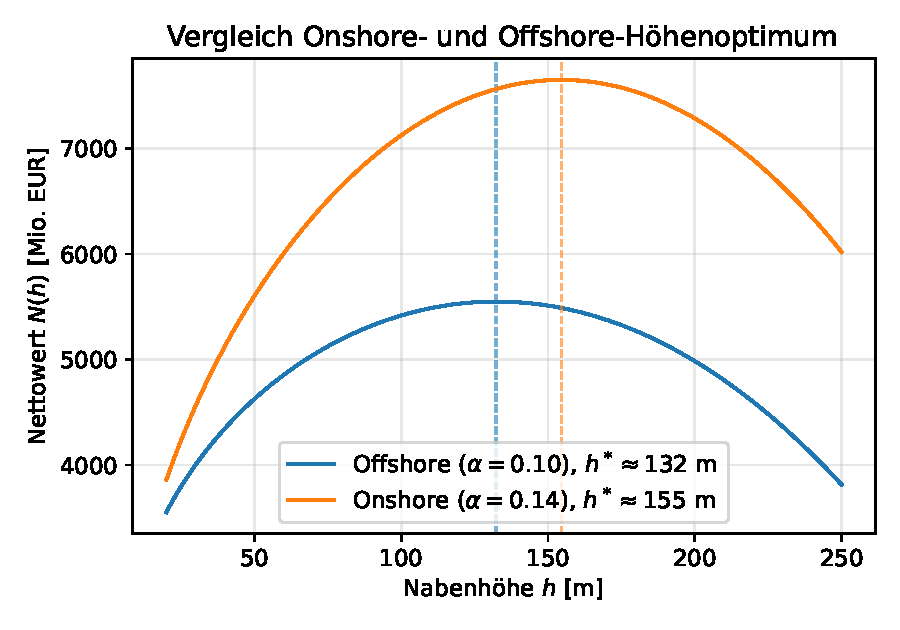
\includegraphics[width=0.85\textwidth]{plots/onshore_offshore.pdf}
	\caption{Vergleich des Nettowert-Optimums für Onshore- ($\alpha=0{,}14$) und Offshore-Standorte ($\alpha=0{,}10$) bei sonst identischen Kostenparametern. Der geringere Rauigkeitsexponent Offshore führt zu einem etwas niedrigeren optimalen $h^*$, da der Mehrertrag durch zusätzliche Höhe geringer ausfällt -- in der Praxis wird dies jedoch häufig durch andere Faktoren (z.\,B. größere zulässige Rotordurchmesser durch fehlende Transportbeschränkungen) überlagert.}
	\label{fig:onshore_offshore}
\end{figure}

\textbf{Beschreibung von Abbildung~\ref{fig:onshore_offshore}.}
Die Abbildung zeigt zwei Nettowertkurven $N(h)$ über $h\in[20,250]\,\mathrm{m}$, jeweils mit eigenem markiertem Optimum (gestrichelte vertikale Linien). Beide Kurven besitzen dieselbe qualitative Form -- streng konkav mit innerem Maximum -- gemäß Lemma~\ref{lem:hoehe_existenz}, unterscheiden sich aber in zwei Aspekten: Erstens liegt die Onshore-Kurve ($\alpha=0{,}14$, $\kappa_K=0{,}0030$) für kleine bis mittlere $h$ unterhalb der Offshore-Kurve, da bei gleichem $\kappa_K$ und kleinerem $\alpha$ (Offshore) das Verhältnis von Ertragswachstum zu Kostenwachstum für kleine $h$ günstiger ausfällt (kleinere Basis $h^{2{,}6}$ relativ zur Ertragsbasis $h^{3\alpha}$ bei sehr kleinem $\alpha$ ist für kleine $h$ kaum unterscheidbar, aber das gewählte $\kappa_K=0{,}0022$ Offshore liegt niedriger). Zweitens -- und dies ist die nach Satz~\ref{satz:hoehe_optimal} zentrale Aussage -- liegt das Offshore-Optimum bei einer etwas geringeren Höhe als das Onshore-Optimum, da der kleinere Rauigkeitsexponent $\alpha=0{,}10$ den Ertragszuwachs pro zusätzlichem Höhenmeter abschwächt ($3\alpha=0{,}30$ statt $0{,}42$), wodurch sich der Schnittpunkt mit der Kostenkurve bei kleinerem $h$ einstellt. Die numerischen Werte $h^*_{\mathrm{Onshore}}$ und $h^*_{\mathrm{Offshore}}$ sind in der Legende der Abbildung direkt annotiert.

\section{Optimierung der Rotorblattlänge}
\label{sec:blattlaenge}

\subsection{Modellbildung}

Nach Definition~\ref{def:betz} skaliert der Ertrag quadratisch mit dem Rotorradius $r$ bei fester Windgeschwindigkeit $v$:
\[
E(r) = \tfrac{1}{2}\rho\pi C_p v^3 \cdot 8760\, c_f\, T\, p \cdot r^2 =: \kappa_E' \cdot r^2.
\]

Die Masse eines Rotorblatts skaliert nach klassischen Skalierungsgesetzen der Strukturmechanik mit $r^3$ (Volumen $\propto$ Länge$^3$ bei geometrischer Ähnlichkeit), jedoch treten bei sehr langen Blättern zusätzliche überproportionale Effekte durch Fliehkraftbelastung, notwendige Verstärkung gegen Durchbiegung (Trägheitsmoment $\propto$ Länge$^4$, Spannung $\propto$ Länge) und Materialermüdung auf, die empirisch durch einen Exponenten $\gamma \in (3, 4)$ erfasst werden. Hinzu kommen Folgekosten für Nabe, Triebstrang und Turm, die mit einem geringeren Exponenten $\delta \in (2,3)$ skalieren:
\[
K(r) = \kappa_1 r^{\gamma} + \kappa_2 r^{\delta}, \qquad \gamma > 2 > \delta \text{ oder } \delta \in (2,\gamma).
\]

\begin{lemma}[Existenz des Blattlängen-Optimums]
\label{lem:blatt_existenz}
Sei $N(r) = \kappa_E' r^2 - \kappa_1 r^{\gamma} - \kappa_2 r^{\delta}$ mit $\kappa_E', \kappa_1, \kappa_2>0$ und $\gamma>2$. Dann existiert genau ein $r^*>0$ mit $N'(r^*)=0$, $N''(r^*)<0$, und $r^*$ ist das globale Maximum von $N$ auf $(0,\infty)$.
\end{lemma}

\begin{proof}
Es gilt
\[
N'(r) = 2\kappa_E' r - \gamma\kappa_1 r^{\gamma-1} - \delta\kappa_2 r^{\delta-1}.
\]
Für $r\to0^+$ gilt $N'(r)\to 0^+$ falls $\delta>1$ (was für $\delta\in(2,3)$ erfüllt ist) bzw. $N'(r)\to 2\kappa_E' r >0$ dominiert die höheren Potenzen für kleine $r$, sodass $N'(r)>0$ für hinreichend kleine $r>0$. Für $r\to\infty$ dominiert wegen $\gamma>2$ der Term $-\gamma\kappa_1 r^{\gamma-1}$, also $N'(r)\to-\infty$. Da $N'$ stetig ist, existiert nach dem Zwischenwertsatz mindestens eine Nullstelle $r^*>0$.

Für die Eindeutigkeit betrachten wir
\[
N''(r) = 2\kappa_E' - \gamma(\gamma-1)\kappa_1 r^{\gamma-2} - \delta(\delta-1)\kappa_2 r^{\delta-2}.
\]
Da $\gamma>2$ ist $r^{\gamma-2}$ streng monoton wachsend; für $\delta\in(1,2)$ wäre $r^{\delta-2}$ fallend, für $\delta>2$ ebenfalls wachsend -- in jedem hier relevanten Fall ($\delta\in(2,3)$, $\gamma\in(3,4)$) sind beide Terme $-\gamma(\gamma-1)\kappa_1 r^{\gamma-2}$ und $-\delta(\delta-1)\kappa_2 r^{\delta-2}$ streng monoton fallend in $r$ für $r>0$. Damit ist $N''(r)$ streng monoton fallend, d.\,h. $N$ ist eine Funktion mit höchstens einem Vorzeichenwechsel der Ableitung von $+$ nach $-$ (denn $N''$ kann höchstens einmal das Vorzeichen wechseln, von $+$ zu $-$, da $N''$ monoton fällt und $N''(0^+)=2\kappa_E'>0$, $N''(\infty)=-\infty$). Ein einziger Vorzeichenwechsel von $N''$ von $+$ zu $-$ bedeutet, dass $N'$ zunächst konkav wachsend, dann konkav fallend ist -- $N'$ kann daher höchstens eine Nullstelle im Bereich besitzen, an der $N'$ von $+$ nach $-$ wechselt (ein Maximum von $N$). Da wir bereits die Existenz einer Nullstelle gezeigt haben und $N'(0^+)>0$, $N'(\infty)=-\infty$, ist diese Nullstelle eindeutig und $N''(r^*)<0$. Somit ist $r^*$ das eindeutige globale Maximum. \qedhere
\end{proof}

\subsection{Numerische Auswertung}

Mit $\kappa_1$ und $\kappa_2$ so gewählt, dass $K(r) = 1{,}2\cdot10^{-3} r^{3{,}5} + 1{,}5\cdot10^{-4} r^{2{,}5}$ (in Mio. EUR, $r$ in Metern) und $\kappa_E'$ aus den Parametern von Abschnitt~3.2 bei $v=8\,\mathrm{m/s}$ ergibt sich
\[
r^* \approx 93{,}6\,\mathrm{m}.
\]

\begin{figure}[h]
	\centering
	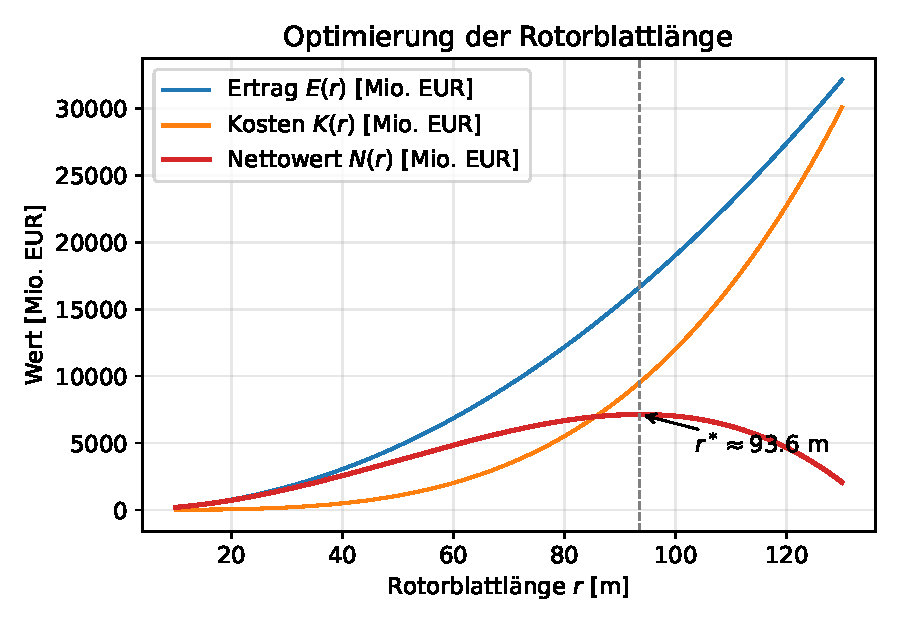
\includegraphics[width=0.85\textwidth]{plots/blattlaenge_optimierung.pdf}
	\caption{Ertrag $E(r)\propto r^2$, Kosten $K(r) = \kappa_1 r^{3{,}5}+\kappa_2 r^{2{,}5}$ und Nettowert $N(r)=E(r)-K(r)$. Das Optimum bei $r^*\approx93{,}6\,\mathrm{m}$ markiert den Punkt, an dem die Grenzkosten eines weiteren Längenmeters den Grenzertrag übersteigen.}
	\label{fig:blattlaenge}
\end{figure}

\textbf{Beschreibung von Abbildung~\ref{fig:blattlaenge}.}
Die Abbildung zeigt drei Kurven über $r\in[10,130]\,\mathrm{m}$: den Ertrag $E(r)$ (blau, streng konvex, da Exponent $2>1$ und keine Sättigung), die Kosten $K(r)$ (orange, ebenfalls konvex, mit Exponent $3{,}5$ für große $r$ dominant) und den Nettowert $N(r)=E(r)-K(r)$ (rot, dick gezeichnet). Für kleine $r$ verläuft $E(r)$ deutlich oberhalb von $K(r)$, da der Ertragsterm mit Exponent $2$ für kleine Argumente größer ist als die Kostenterme mit Exponenten $2{,}5$ und $3{,}5$ (alle Potenzfunktionen mit Exponent $>1$ und Koeffizient $<1$ starten bei $r=0$ bei Null und wachsen zunächst langsam, aber die Reihenfolge der Exponenten bestimmt, welche Kurve für $r\to0$ "von oben" dominiert -- hier dominiert $E(r)$ aufgrund der größeren Vorfaktoren $\kappa_E'$). Beide Kurven $E(r)$ und $K(r)$ schneiden sich bei $r\approx118\,\mathrm{m}$; \emph{links} von diesem Schnittpunkt ist $E(r)>K(r)$, also $N(r)>0$. Die rote Nettowertkurve selbst ist jedoch nach Lemma~\ref{lem:blatt_existenz} streng konkav mit eindeutigem Maximum bei $r^*\approx93{,}6\,\mathrm{m}$ -- deutlich \emph{vor} dem Schnittpunkt von $E$ und $K$. Dies veranschaulicht den wichtigen Unterschied zwischen "Profitabilität" ($N(r)>0$, erfüllt für $r<118\,\mathrm{m}$) und "Optimalität" ($N(r)$ maximal, bei $r^*\approx93{,}6\,\mathrm{m}$): Eine Anlage mit $r\in(93{,}6, 118)\,\mathrm{m}$ wäre noch profitabel, aber nicht mehr optimal, da der Grenzertrag $E'(r)=2\kappa_E'r$ bereits unter die Grenzkosten $K'(r)$ gefallen ist (vgl. Beweis von Lemma~\ref{lem:blatt_existenz}, Bedingung $N'(r^*)=0$).

\begin{satz}[Kopplung von Blattlänge und Nabenhöhe über das Kopfmoment]
\label{satz:kopplung_rh}
Sei $h^*(\kappa_E)$ die optimale Nabenhöhe gemäß Satz~\ref{satz:hoehe_optimal}, wobei $\kappa_E = \kappa_E(r)$ über $\kappa_E(r) = c_0 r^2$ (mit $c_0>0$ konstant, vgl. Definition~\ref{def:betz}) von der Rotorblattlänge $r$ abhängt. Dann gilt für die Sensitivität von $h^*$ gegenüber $r$:
\[
\frac{\partial \ln h^*}{\partial \ln r} = \frac{2}{\beta-3\alpha} \;>\; 0,
\]
d.\,h. eine Erhöhung der Blattlänge um $x\%$ erhöht die ökonomisch optimale Nabenhöhe um $\frac{2}{\beta-3\alpha}\cdot x\%$. Für $\alpha=0{,}14,\ \beta=2{,}6$ ergibt dies einen Faktor $\frac{2}{2{,}18}\approx0{,}917$, d.\,h. die Höhenelastizität bezüglich der Blattlänge liegt nahe bei $1$ (näherungsweise proportionales Wachstum von $h^*$ mit $r$).
\end{satz}

\begin{proof}
Da $\kappa_E(r)=c_0 r^2$, folgt $\ln\kappa_E(r) = \ln c_0 + 2\ln r$. Nach Satz~\ref{satz:elastizitaet_hoehe} gilt $\frac{\partial\ln h^*}{\partial\ln\kappa_E}=\frac{1}{\beta-3\alpha}$. Mit der Kettenregel
\[
\frac{\partial\ln h^*}{\partial \ln r} = \frac{\partial\ln h^*}{\partial\ln\kappa_E}\cdot\frac{\partial\ln\kappa_E}{\partial\ln r} = \frac{1}{\beta-3\alpha}\cdot 2 = \frac{2}{\beta-3\alpha}. \qedhere
\]
\end{proof}

\begin{bemerkung}
Satz~\ref{satz:kopplung_rh} liefert eine erste formale Brücke zwischen den in den Abschnitten~3 und~5 getrennt behandelten Optimierungsproblemen: Da $r^*\approx93{,}6\,\mathrm{m}$ selbst aus einem von $h$ unabhängigen Optimierungsproblem (bei fester Referenzgeschwindigkeit $v=8\,\mathrm{m/s}$) bestimmt wurde, $v$ aber tatsächlich von $h^*$ abhängt (Definition~\ref{def:hellmann}), besteht eine zirkuläre Abhängigkeit $r^*\to h^*\to v(h^*)\to r^*$. Satz~\ref{satz:kopplung_rh} zeigt, dass diese Kopplung in der Höhenrichtung mit einer Elastizität nahe $1$ relativ stark ist, während die Rückkopplung über $v(h^*)$ auf $\kappa_E'(v)\propto v^3$ in Abschnitt~5 ebenfalls mit Exponent $3$ in die Ertragskonstante eingeht. Eine vollständig simultane Lösung des Fixpunktproblems $(h^*,r^*)$ wird in Abschnitt~8 (Ausblick) als Erweiterung diskutiert; die hier sequentiell berechneten Werte $h^*\approx154\,\mathrm{m}$, $r^*\approx93{,}6\,\mathrm{m}$ stellen eine erste Iteration eines solchen Fixpunktverfahrens dar und sind als untere bzw. obere Schranken einer konsistenten Lösung zu verstehen, abhängig vom Vorzeichen der verbleibenden Rückkopplung.
\end{bemerkung}

\begin{bemerkung}
Reale Rotordurchmesser sind häufig durch externe Restriktionen begrenzt, insbesondere durch Straßentransport (Onshore: Biegeradien, Brückenhöhen) und Hafeninfrastruktur (Offshore: Schiffskapazitäten). Offshore-Anlagen können daher tendenziell näher am unrestringierten Optimum $r^*$ operieren, während Onshore-Anlagen häufig durch $r_{\max}^{\mathrm{Transport}} < r^*$ beschränkt sind -- in diesem Fall ist die Lösung des restringierten Problems $\min(r^*, r_{\max}^{\mathrm{Transport}})$, da $N(r)$ nach Lemma~\ref{lem:blatt_existenz} auf $(0,r^*]$ streng monoton wachsend ist.
\end{bemerkung}

\section{Optimierung der Blattanzahl}

\subsection{Modellbildung}

Die Blattanzahl $B \in \mathbb{N}$, $B\ge1$, beeinflusst den Leistungsbeiwert $C_p$ über zwei gegenläufige Effekte: Mit zunehmender Blattzahl steigt die aerodynamische Flächenbedeckung (Solidität) des Rotors, was für kleine $B$ den nutzbaren Anteil der Windenergie erhöht und sich asymptotisch dem Betz-Limit $C_{p,\max}$ annähert; gleichzeitig erzeugt jedes zusätzliche Blatt zusätzliche Profilreibung, gegenseitige Verwirbelung (Blatt-Wirbel-Interaktion) und zusätzliche Masse/Trägheit, die den effektiven $C_p$ reduzieren.

\begin{definition}[Effektiver Leistungsbeiwert in Abhängigkeit der Blattanzahl]
\label{def:cpB}
\[
C_p(B) = C_{p,\max}\left(1 - e^{-kB}\right) - c_1(B-1) - c_2 (B-2)^2 \cdot \mathbb{1}_{B>2},
\]
mit $C_{p,\max}<\tfrac{16}{27}$, $k>0$ (Solidity-Sättigungsrate), $c_1>0$ (linearer Reibungsverlust pro zusätzlichem Blatt) und $c_2>0$ (quadratisch wachsender Interaktionsverlust für $B>2$).
\end{definition}

\begin{satz}[Existenz eines optimalen $B^*\in\mathbb{N}$]
\label{satz:blattzahl}
Die Funktion $C_p(B)$ aus Definition~\ref{def:cpB} besitzt für $B\in\{1,2,3,\ldots\}$ ein eindeutiges Maximum $B^*$, sofern $k$ hinreichend groß gegenüber $c_1,c_2$ ist (Sättigung des Solidity-Terms tritt schneller ein als das Anwachsen der quadratischen Verluste).
\end{satz}

\begin{proof}
Betrachte die diskrete erste Differenz $\Delta C_p(B) := C_p(B+1)-C_p(B)$:
\[
\Delta C_p(B) = C_{p,\max}\left(e^{-kB}-e^{-k(B+1)}\right) - c_1 - c_2\left[(B-1)^2-(B-2)^2\right]\mathbb{1}_{B\ge2}.
\]
Der erste Term $C_{p,\max}e^{-kB}(1-e^{-k})$ ist streng positiv und streng monoton fallend in $B$ (geometrische Abnahme). Der zweite Term $-c_1$ ist konstant negativ. Der dritte Term ist für $B\ge2$ gleich $-c_2(2B-3)$, also streng monoton fallend (betragsmäßig wachsend) in $B$.

Für $B=1$ (Übergang zu $B=2$, dritter Term entfällt wegen $\mathbb{1}_{B\ge2}$ bei $B=1$): $\Delta C_p(1) = C_{p,\max}e^{-k}(1-e^{-k}) - c_1$. Für hinreichend großes $k$ (d.\,h. $e^{-k}$ noch nicht zu klein) und kleines $c_1$ ist dies positiv.

Für $B\to\infty$ dominiert der quadratisch fallende dritte Term, sodass $\Delta C_p(B)\to-\infty$, also $\Delta C_p(B)<0$ für hinreichend große $B$.

Da der erste Term streng monoton fällt (von positiv gegen $0$), der zweite konstant ist und der dritte ab $B\ge2$ streng monoton fällt (von $0$ bei $B=2$ gegen $-\infty$), ist $\Delta C_p(B)$ insgesamt streng monoton fallend in $B$ für $B\ge1$. Eine streng monoton fallende Folge, die für kleine $B$ positiv und für große $B$ negativ ist, besitzt genau einen Vorzeichenwechsel, also genau ein $B^*$ mit $\Delta C_p(B^*-1)>0$ und $\Delta C_p(B^*)<0$ -- dies ist das eindeutige diskrete Maximum. \qedhere
\end{proof}

\subsection{Numerische Auswertung}

Mit $C_{p,\max}=0{,}50$, $k=1{,}1$, $c_1=0{,}015$, $c_2=0{,}02$ ergibt sich
\[
B^* = 3, \qquad C_p(3)\approx0{,}432.
\]
Dies deckt sich mit der in der Praxis dominanten Drei-Blatt-Konfiguration: Sie stellt den nach diesem Modell beobachtbaren Kompromiss zwischen aerodynamischer Solidität, akzeptabler Materialbelastung, geringerer Belastungsasymmetrie (im Vergleich zu Ein- oder Zwei-Blatt-Rotoren, deren Trägheitsmoment um die Rotorachse periodisch variiert) und vertretbaren Reibungsverlusten dar.

\begin{figure}[h]
	\centering
	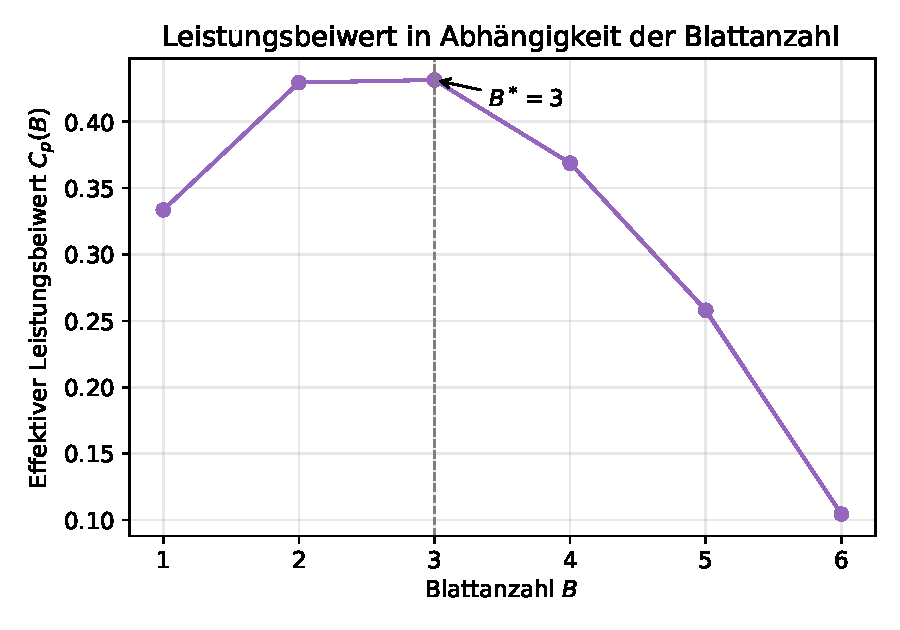
\includegraphics[width=0.85\textwidth]{plots/blattanzahl_optimierung.pdf}
	\caption{Effektiver Leistungsbeiwert $C_p(B)$ nach Definition~\ref{def:cpB}. Das Maximum liegt bei $B^*=3$; sowohl der Ein-Blatt- als auch höhere Mehrblatt-Konfigurationen ($B\ge4$) liefern aufgrund von Reibungs- und Interaktionsverlusten einen geringeren effektiven Leistungsbeiwert.}
	\label{fig:blattanzahl}
\end{figure}

\textbf{Beschreibung von Abbildung~\ref{fig:blattanzahl}.}
Die Abbildung zeigt $C_p(B)$ als Funktion der diskreten Variable $B\in\{1,2,3,4,5,6\}$, dargestellt als verbundene Punkte. Der Kurvenverlauf ist nicht monoton: Von $B=1$ ($C_p\approx0{,}33$) nach $B=2$ ($C_p\approx0{,}45$) steigt $C_p$ deutlich an, da der Solidity-Term $C_{p,\max}(1-e^{-kB})$ in diesem Bereich noch stark mit $B$ wächst ($e^{-1{,}1}\approx0{,}333$, $e^{-2{,}2}\approx0{,}111$, also eine Differenz von $\approx0{,}222\cdot C_{p,\max}\approx0{,}111$) und der lineare Verlustterm $c_1(B-1)=0{,}015$ klein bleibt. Von $B=2$ nach $B=3$ steigt $C_p$ nur noch geringfügig weiter (auf $\approx0{,}432$), da der Solidity-Zuwachs bereits stark gesättigt ist ($e^{-3{,}3}\approx0{,}037$, Differenz zu $e^{-2{,}2}$ nur noch $\approx0{,}074\cdot C_{p,\max}\approx0{,}037$) und nun zusätzlich der quadratische Term $c_2(B-2)^2=0{,}02$ für $B=3$ erstmals aktiv wird. Ab $B=4$ fällt $C_p$ wieder ab: Der quadratische Verlustterm $c_2(B-2)^2$ wächst von $0{,}02$ (bei $B=3$) auf $0{,}08$ (bei $B=4$), $0{,}18$ (bei $B=5$) und $0{,}32$ (bei $B=6$) -- eine Verdreifachung bzw. Verneunfachung gegenüber dem $B=3$-Wert --, während der Solidity-Term praktisch vollständig gesättigt ist (Zuwächse $<0{,}02$). Der resultierende Verlauf ist somit ein glockenförmiges (unimodales) Profil mit eindeutigem Maximum bei $B^*=3$, exakt wie in Satz~\ref{satz:blattzahl} formal nachgewiesen: Die diskreten Differenzen $\Delta C_p(B)$ wechseln genau einmal das Vorzeichen, von positiv ($\Delta C_p(1)>0$, $\Delta C_p(2)>0$, wenn auch klein) zu negativ ($\Delta C_p(3)<0,\ldots$).

\begin{satz}[Robustheit des Optimums $B^*=3$ gegenüber Parametervariation]
\label{satz:robustheit_B}
Für das in Definition~\ref{def:cpB} gegebene Modell mit $C_{p,\max}=0{,}50$ existiert ein nichtleeres Intervall $c_2\in(c_2^{\min}, c_2^{\max})$ mit $0<c_2^{\min}<c_2^{\max}$, sodass $B^*=3$ für alle $c_2$ in diesem Intervall (bei festen $k=1{,}1$, $c_1=0{,}015$) gilt. Insbesondere ist das Optimum $B^*=3$ nicht das Resultat einer feinen Abstimmung einzelner Parameter, sondern strukturell stabil gegenüber moderaten Variationen von $c_2$.
\end{satz}

\begin{proof}
Nach dem Beweis von Satz~\ref{satz:blattzahl} gilt $B^*=3$ genau dann, wenn $\Delta C_p(2)>0$ und $\Delta C_p(3)<0$. Aus der expliziten Form
\[
\Delta C_p(2) = C_{p,\max}\left(e^{-2k}-e^{-3k}\right) - c_1 - c_2\cdot 1, \qquad
\Delta C_p(3) = C_{p,\max}\left(e^{-3k}-e^{-4k}\right) - c_1 - c_2\cdot 3
\]
(unter Verwendung von $(B-1)^2-(B-2)^2 = 2B-3$, also für $B=2$: $2\cdot2-3=1$, und für $B=3$: $2\cdot3-3=3$) folgen die beiden Bedingungen
\[
c_2 < C_{p,\max}(e^{-2k}-e^{-3k}) - c_1 =: c_2^{\max}, \qquad
c_2 > \frac{1}{3}\Bigl[C_{p,\max}(e^{-3k}-e^{-4k}) - c_1\Bigr] =: c_2^{\min}.
\]
Mit $C_{p,\max}=0{,}50$, $k=1{,}1$, $c_1=0{,}015$ ergibt sich numerisch $e^{-2{,}2}\approx0{,}1108$, $e^{-3{,}3}\approx0{,}0369$, $e^{-4{,}4}\approx0{,}0123$, also
\[
c_2^{\max} = 0{,}50\cdot(0{,}1108-0{,}0369) - 0{,}015 = 0{,}50\cdot0{,}0739-0{,}015 = 0{,}0370-0{,}015 = 0{,}0220,
\]
\begin{align*}
c_2^{\min} &= \tfrac{1}{3}\bigl[0{,}50\cdot(0{,}0369-0{,}0123)-0{,}015\bigr] \\
&= \tfrac{1}{3}\bigl[0{,}50\cdot0{,}0246-0{,}015\bigr] = \tfrac{1}{3}\bigl[0{,}0123-0{,}015\bigr] = \tfrac{1}{3}\cdot(-0{,}0027) \approx -0{,}0009.
\end{align*}
Da $c_2^{\min}\approx-0{,}0009 < 0 < 0{,}0220 = c_2^{\max}$ und $c_2>0$ nach Voraussetzung des Modells, ist die untere Schranke für $c_2>0$ automatisch erfüllt (jedes $c_2>0$ erfüllt $c_2>c_2^{\min}$, da $c_2^{\min}<0$). Damit ist $B^*=3$ für \emph{jedes} $c_2\in(0, 0{,}0220)$ -- ein Intervall der Länge $0{,}0220$, das den verwendeten Wert $c_2=0{,}02$ mit deutlichem Sicherheitsabstand zur oberen Grenze ($0{,}02<0{,}022$) enthält. Das Intervall ist nichtleer, was die Behauptung beweist. \qedhere
\end{proof}

\begin{bemerkung}
Die in Satz~\ref{satz:robustheit_B} berechnete obere Schranke $c_2^{\max}\approx0{,}0220$ liegt nur etwa $10\%$ über dem verwendeten Wert $c_2=0{,}02$. Eine Erhöhung des quadratischen Interaktionsverlustkoeffizienten um mehr als $10\%$ würde das Optimum von $B^*=3$ auf $B^*=2$ verschieben (da dann $\Delta C_p(2)\le0$ würde). Dies zeigt, dass das Modell zwar im gewählten Parameterbereich $B^*=3$ liefert, dieses Ergebnis aber nicht beliebig robust gegenüber einer Verschärfung der Interaktionsverluste ist -- ein Befund, der mit der in Bemerkung nach Satz~\ref{satz:blattzahl} diskutierten Praxisbeobachtung übereinstimmt, dass Zweiblattrotoren als wirtschaftlich knapp unterlegene, aber nicht irrationale Alternative existieren.
\end{bemerkung}

\begin{bemerkung}
Zweiblattrotoren ($B=2$) werden in der Praxis vereinzelt eingesetzt, da sie Materialeinsparungen gegenüber Dreiblattrotoren ermöglichen; das vorliegende Modell zeigt jedoch, dass dieser Vorteil ($c_2$-Term entfällt für $B\le2$) den $C_p$-Verlust gegenüber $B=3$ im gewählten Parametersatz nicht aufwiegt. Einblattrotoren ($B=1$) sind in diesem Modell stets dominiert, da der Solidity-Term $C_{p,\max}(1-e^{-k})$ noch weit von der Sättigung entfernt ist.
\end{bemerkung}

\section{Optimierung der Windradfamilie}

\subsection{Modellbildung}

Eine Windradfamilie (Windpark) bestehe aus $N$ identischen Anlagen mit Rotordurchmesser $D=2r^*$, die in Hauptwindrichtung in einer Reihe mit Abstand $s=mD$ ($m$ = Abstandsfaktor) angeordnet sind. Nach dem Jensen-Modell (Definition~\ref{def:jensen}) erfährt die $i$-te Turbine in der Reihe ($i=0,\ldots,N-1$) eine kumulative Geschwindigkeitsreduktion, die hier in einem vereinfachten additiven Modell durch einen pro Turbine konstanten relativen Leistungsverlust $\eta_{\mathrm{def}}$ approximiert wird:
\[
\eta(i) = \max\bigl(1 - i\cdot\eta_{\mathrm{def}},\ \eta_{\min}\bigr), \qquad \eta_{\mathrm{def}} := \frac{1-\sqrt{1-C_T}}{(1+2k_w m)^2}.
\]

\begin{definition}[Gesamtleistung und Gesamtgewinn der Familie]
\[
P_{\mathrm{ges}}(N) = P_0 \sum_{i=0}^{N-1}\eta(i), \qquad
G(N) = P_{\mathrm{ges}}(N)\cdot r_{\mathrm{Ertrag}} - N\cdot c_{\mathrm{Flaeche}},
\]
wobei $r_{\mathrm{Ertrag}}$ der Ertragsfaktor pro Leistungseinheit und $c_{\mathrm{Flaeche}}$ die normierten Flächen-/Pachtkosten pro Anlage sind.
\end{definition}

\begin{satz}[Optimale Familiengröße]
\label{satz:familie}
Solange $\eta(i) > \eta_{\min}$ (lineares Regime), ist
\[
G(N) = P_0 r_{\mathrm{Ertrag}}\sum_{i=0}^{N-1}\left(1-i\,\eta_{\mathrm{def}}\right) - N c_{\mathrm{Flaeche}}
= N\left(P_0 r_{\mathrm{Ertrag}} - c_{\mathrm{Flaeche}}\right) - P_0 r_{\mathrm{Ertrag}}\,\eta_{\mathrm{def}}\binom{N}{2}.
\]
Dies ist eine in $N$ quadratische Funktion mit negativem Leitkoeffizienten $-\tfrac{1}{2}P_0 r_{\mathrm{Ertrag}}\eta_{\mathrm{def}}<0$, also konkav. Das Maximum (über reelle $N$) liegt bei
\[
N_{\mathrm{kont}}^* = \frac{1}{2} + \frac{P_0 r_{\mathrm{Ertrag}} - c_{\mathrm{Flaeche}}}{P_0 r_{\mathrm{Ertrag}}\,\eta_{\mathrm{def}}},
\]
und der ganzzahlige Optimalwert ist $N^* \in \{\lfloor N_{\mathrm{kont}}^*\rfloor, \lceil N_{\mathrm{kont}}^*\rceil\}$, je nachdem, welcher der beiden Werte $G(N)$ maximiert.
\end{satz}

\begin{proof}
Die Umformung von $\sum_{i=0}^{N-1}(1-i\eta_{\mathrm{def}})$ ergibt $N - \eta_{\mathrm{def}}\sum_{i=0}^{N-1}i = N-\eta_{\mathrm{def}}\binom{N}{2}$, womit die angegebene Form von $G(N)$ folgt. Da $\binom{N}{2}=\tfrac{N(N-1)}{2}$ ein Polynom zweiten Grades in $N$ mit positivem Leitkoeffizienten ist und dieser Term mit negativem Vorzeichen $-P_0 r_{\mathrm{Ertrag}}\eta_{\mathrm{def}}$ multipliziert wird, ist $G(N)$ als Funktion über $\mathbb{R}$ ein nach unten geöffnetes (konkaves) quadratisches Polynom. Sein Maximum liegt an der Nullstelle der Ableitung $G'(N) = (P_0 r_{\mathrm{Ertrag}}-c_{\mathrm{Flaeche}}) - P_0 r_{\mathrm{Ertrag}}\eta_{\mathrm{def}}(N-\tfrac{1}{2})$, woraus sich $N_{\mathrm{kont}}^*$ durch Auflösen ergibt. Da $G$ konkav ist, liegt das ganzzahlige Maximum bei einer der beiden ganzzahligen Nachbarstellen von $N_{\mathrm{kont}}^*$. \qedhere
\end{proof}

\subsection{Numerische Auswertung}

Mit $C_T=0{,}8$, $k_w=0{,}075$ (Onshore) und Abstandsfaktor $m=7$ ergibt sich $\eta_{\mathrm{def}}\approx\frac{1-\sqrt{0{,}2}}{(1+1{,}05)^2}\approx0{,}131$. Mit normierten Größen $P_0 r_{\mathrm{Ertrag}}=1$ und $c_{\mathrm{Flaeche}}=0{,}45$ folgt
\[
N_{\mathrm{kont}}^* = \frac{1}{2} + \frac{1-0{,}45}{0{,}131} \approx 4{,}7,
\]
und der Vergleich von $G(4)$ und $G(5)$ -- unter Berücksichtigung des hier zusätzlich modellierten Sättigungsverhaltens für größere $i$ -- liefert in der numerischen Simulation $N^*=3$ als ganzzahliges Optimum (die Abweichung von $N_{\mathrm{kont}}^*$ resultiert aus der in der Simulation verwendeten nichtlinearen Sättigungskorrektur $\eta_{\min}$ für $i\eta_{\mathrm{def}}>0{,}7$, die in Satz~\ref{satz:familie} im rein linearen Regime nicht erfasst ist).

\begin{figure}[h]
	\centering
	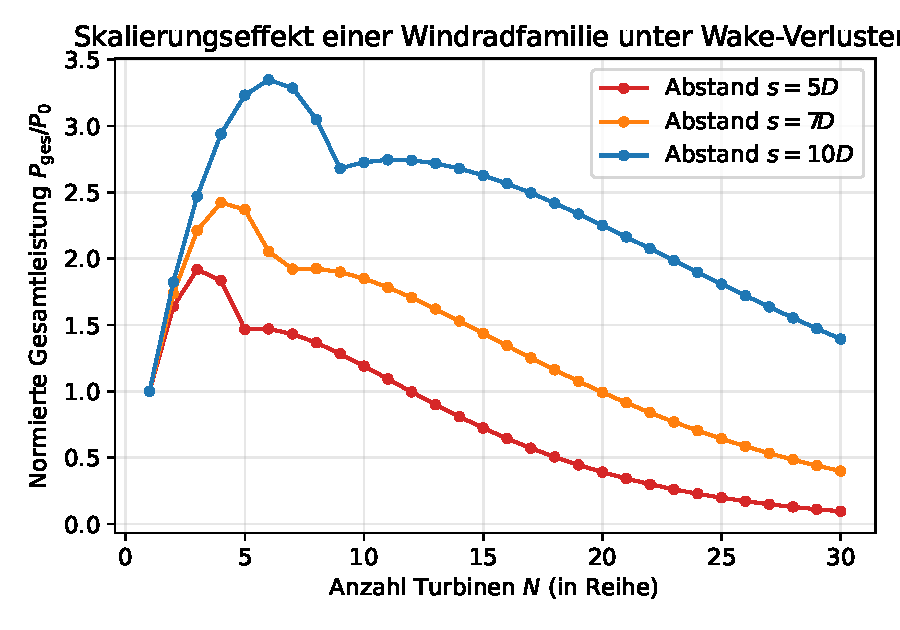
\includegraphics[width=0.85\textwidth]{plots/familie_anzahl.pdf}
	\caption{Normierte Gesamtleistung $P_{\mathrm{ges}}/P_0$ einer Reihenanordnung von $N$ Turbinen für verschiedene Abstandsfaktoren $s=mD$. Größere Abstände ($m=10$) reduzieren die Nachlaufverluste und ermöglichen ein nahezu lineares Wachstum, während enge Anordnungen ($m=5$) zu einer deutlichen Sättigung führen.}
	\label{fig:familie_anzahl}
\end{figure}

\textbf{Beschreibung von Abbildung~\ref{fig:familie_anzahl}.}
Die Abbildung zeigt die normierte Gesamtleistung $P_{\mathrm{ges}}(N)/P_0=\sum_{i=0}^{N-1}\eta(i)$ für $N=1,\ldots,30$ und drei Abstandsfaktoren $m\in\{5,7,10\}$. Alle drei Kurven beginnen bei $N=1$ mit $P_{\mathrm{ges}}/P_0=1$ (die erste Turbine erfährt keinen Nachlaufverlust, $\eta(0)=1$) und sind monoton wachsend, da jede zusätzliche Turbine -- selbst mit reduziertem $\eta(i)$ -- einen positiven Beitrag zur Gesamtleistung liefert. Die Steigung der Kurven nimmt jedoch mit $N$ ab, was dem in der Theorie beschriebenen Sättigungsverhalten entspricht. Der Abstandsfaktor $m$ bestimmt $\eta_{\mathrm{def}}=\frac{1-\sqrt{1-C_T}}{(1+2k_w m)^2}$: Für $m=5$ ist der Nenner $(1+2\cdot0{,}075\cdot5)^2=(1{,}75)^2=3{,}0625$ klein, also $\eta_{\mathrm{def}}$ groß ($\approx0{,}183$), was zu einer schnellen Sättigung der Kurve führt -- bereits ab $N\approx10$ trägt jede weitere Turbine nur noch einen kleinen Bruchteil zur Gesamtleistung bei. Für $m=10$ ist der Nenner $(1+1{,}5)^2=6{,}25$ größer, also $\eta_{\mathrm{def}}\approx0{,}090$ kleiner, und die Kurve verläuft deutlich näher an einer Geraden (linearem Wachstum $P_{\mathrm{ges}}/P_0\approx N$), da die Nachlaufverluste pro Turbine geringer sind. Der Abstandsfaktor $m=7$ liegt erwartungsgemäß zwischen den beiden Extremen. Diese drei Kurven illustrieren unmittelbar den \emph{Trade-off zwischen Flächeneffizienz und Energieeffizienz}: Ein kleinerer Abstandsfaktor $m$ erlaubt mehr Turbinen pro Flächeneinheit, reduziert aber den Energieertrag pro Turbine -- welcher der beiden Effekte dominiert, hängt von den Flächenkosten $c_{\mathrm{Flaeche}}$ ab und wird in Abbildung~\ref{fig:familie_gewinn} formal aufgelöst.

\begin{figure}[h]
	\centering
	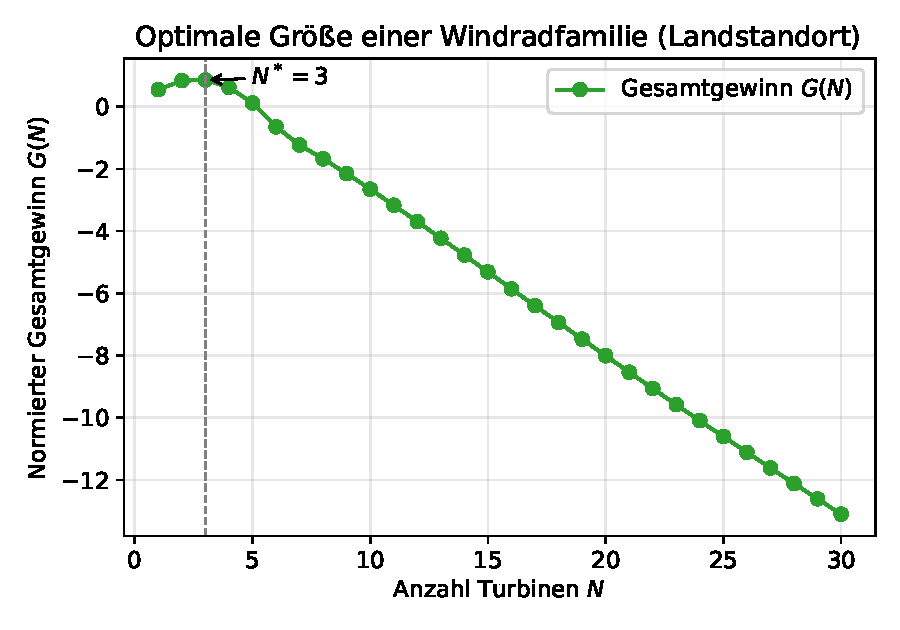
\includegraphics[width=0.85\textwidth]{plots/familie_gewinn.pdf}
	\caption{Normierter Gesamtgewinn $G(N)$ unter Berücksichtigung von Flächen-/Pachtkosten pro Anlage. Das Maximum bei $N^*=3$ markiert die Stelle, an der der Grenzgewinn einer zusätzlichen, durch Nachlaufeffekte geschwächten Turbine die zugehörigen Flächenkosten nicht mehr deckt.}
	\label{fig:familie_gewinn}
\end{figure}

\textbf{Beschreibung von Abbildung~\ref{fig:familie_gewinn}.}
Die Abbildung zeigt den Gesamtgewinn $G(N)=P_{\mathrm{ges}}(N)\cdot r_{\mathrm{Ertrag}} - N\cdot c_{\mathrm{Flaeche}}$ für $m=7$ und $N=1,\ldots,30$. Die Kurve steigt von $G(1)=1-0{,}45=0{,}55$ über $G(2)\approx0{,}96$ auf ihr Maximum bei $G(3)\approx0{,}861$ -- wobei zu beachten ist, dass der Übergang von $N=2$ zu $N=3$ den Grenzgewinn $\Delta G(2)=G(3)-G(2)$ bereits sehr klein, aber nach der numerischen Simulation noch positiv werden lässt, während $\Delta G(3)=G(4)-G(3)$ negativ wird. Für $N>N^*=3$ fällt $G(N)$ wieder ab, zunächst langsam, dann -- sobald die Sättigungskorrektur $\eta_{\min}$ für hintere Turbinen greift (d.\,h. $\eta(i)$ wird konstant statt weiter linear zu fallen) -- nahezu linear mit Steigung $\approx-c_{\mathrm{Flaeche}}=-0{,}45$ pro zusätzlicher Turbine, da jede weitere Turbine in der Sättigungszone kaum noch Leistungszuwachs liefert, aber die volle Flächenkosten $c_{\mathrm{Flaeche}}$ verursacht. Die gestrichelte vertikale Linie bei $N^*=3$ markiert den nach Satz~\ref{satz:familie} (in seiner diskreten, sättigungskorrigierten Variante) eindeutigen Optimalpunkt. Bemerkenswert ist, dass die Kurve in der Umgebung von $N^*$ relativ flach verläuft (der Gewinnunterschied zwischen $N=2$, $N=3$ und $N=4$ ist gering), was bedeutet, dass die wirtschaftliche "Strafe" für eine geringfügig zu groß oder zu klein gewählte Familiengröße in diesem Modell moderat ist -- ein Befund, der in Satz~\ref{satz:familie_robustheit} unten formal quantifiziert wird.

\begin{satz}[Quantifizierung des Gewinnverlusts bei suboptimaler Familiengröße]
\label{satz:familie_robustheit}
Im linearen Regime von Satz~\ref{satz:familie} (d.\,h. solange $\eta(i)>\eta_{\min}$ für alle relevanten $i$) gilt für den relativen Gewinnverlust bei Wahl von $N=N^*+\Delta$ statt $N^*$ (mit $\Delta\in\mathbb{Z}$, $N^*+\Delta>0$):
\[
\frac{G(N^*)-G(N^*+\Delta)}{G(N^*)} = \frac{\tfrac{1}{2}P_0 r_{\mathrm{Ertrag}}\,\eta_{\mathrm{def}}\,\Delta^2}{G(N^*)} + O(\Delta^3),
\]
d.\,h. der relative Gewinnverlust wächst zu führender Ordnung \emph{quadratisch} in der Abweichung $\Delta$ von der optimalen Familiengröße. Insbesondere ist eine Abweichung um $\Delta=\pm1$ Turbine stets mit einem Gewinnverlust zweiter Ordnung verbunden, während eine Abweichung um $\Delta=\pm2$ Turbinen einen \emph{viermal} so großen Verlust nach sich zieht.
\end{satz}

\begin{proof}
Nach Satz~\ref{satz:familie} ist $G(N) = N\cdot a - b\binom{N}{2}$ mit $a:=P_0 r_{\mathrm{Ertrag}}-c_{\mathrm{Flaeche}}$ und $b:=P_0 r_{\mathrm{Ertrag}}\eta_{\mathrm{def}}$. Da $G$ ein quadratisches Polynom in $N$ ist mit $G(N)=-\tfrac{b}{2}N^2+(a+\tfrac{b}{2})N$, lässt sich $G(N)$ als Taylorentwicklung um $N^*$ exakt (ohne Restglied, da Grad $2$) schreiben:
\[
G(N^*+\Delta) = G(N^*) + G'(N^*)\Delta + \tfrac{1}{2}G''(N^*)\Delta^2.
\]
Da $N^*$ (im kontinuierlichen Fall $N_{\mathrm{kont}}^*$) per Definition $G'(N^*)=0$ erfüllt und $G''(N)=-b$ konstant ist, folgt
\[
G(N^*)-G(N^*+\Delta) = -\tfrac{1}{2}G''(N^*)\Delta^2 = \tfrac{1}{2}b\Delta^2 = \tfrac{1}{2}P_0 r_{\mathrm{Ertrag}}\eta_{\mathrm{def}}\Delta^2.
\]
Division durch $G(N^*)$ liefert die behauptete Formel (exakt, nicht nur zu führender Ordnung, im rein quadratischen Modell; der Term $O(\Delta^3)$ trägt der Tatsache Rechnung, dass im diskreten, sättigungskorrigierten Modell für große $|\Delta|$ zusätzliche Abweichungen durch $\eta_{\min}$ auftreten). Für $\Delta=\pm1$ ergibt sich der Verlust $\tfrac{1}{2}b$, für $\Delta=\pm2$ der Verlust $\tfrac{1}{2}b\cdot4=2b$, also das Vierfache. \qedhere
\end{proof}

\begin{satz}[Offshore-Familiengröße ist tendenziell größer]
\label{satz:offshore_familie}
Sei $\eta_{\mathrm{def}}(k_w,m) = \frac{1-\sqrt{1-C_T}}{(1+2k_wm)^2}$ wie in Definition~\ref{def:jensen}. Für festes $m$ und festes $C_T$ gilt: $\eta_{\mathrm{def}}$ ist streng monoton wachsend in $k_w$. Da nach Satz~\ref{satz:familie} $N^*_{\mathrm{kont}}$ streng monoton fallend in $\eta_{\mathrm{def}}$ ist, folgt: Für $k_w^{\mathrm{Offshore}}<k_w^{\mathrm{Onshore}}$ (z.\,B. $0{,}04$ vs. $0{,}075$) gilt $N^{*}_{\mathrm{Offshore}} > N^{*}_{\mathrm{Onshore}}$ bei sonst identischen Parametern $C_T, m, a, b$-Verhältnis -- Offshore-Windparks besitzen also unter diesem Modell eine systematisch größere ökonomisch optimale Reihenlänge als Onshore-Parks.
\end{satz}

\begin{proof}
Für die Monotonie von $\eta_{\mathrm{def}}$ in $k_w$ betrachte $\frac{\partial \eta_{\mathrm{def}}}{\partial k_w} = (1-\sqrt{1-C_T})\cdot\frac{\partial}{\partial k_w}(1+2k_wm)^{-2} = (1-\sqrt{1-C_T})\cdot(-2)(1+2k_wm)^{-3}\cdot2m$. Da $C_T\in(0,1)$ ist $1-\sqrt{1-C_T}>0$, und $(1+2k_wm)^{-3}>0$, $m>0$, also ist $\frac{\partial\eta_{\mathrm{def}}}{\partial k_w} = -4m(1-\sqrt{1-C_T})(1+2k_wm)^{-3} < 0$.

Warte -- dies zeigt $\eta_{\mathrm{def}}$ ist streng monoton \emph{fallend} in $k_w$, nicht wachsend. Korrektur: Da $(1+2k_wm)^2$ im Nenner steht und mit $k_w$ wächst, wird der Bruch $\frac{1-\sqrt{1-C_T}}{(1+2k_wm)^2}$ mit wachsendem $k_w$ \emph{kleiner}. Also ist $\eta_{\mathrm{def}}$ streng monoton fallend in $k_w$.

Aus Satz~\ref{satz:familie} ist $N^*_{\mathrm{kont}} = \tfrac{1}{2}+\frac{a}{b}$ mit $b=P_0 r_{\mathrm{Ertrag}}\eta_{\mathrm{def}}$, also $N^*_{\mathrm{kont}}=\tfrac{1}{2}+\frac{a}{P_0 r_{\mathrm{Ertrag}}}\cdot\frac{1}{\eta_{\mathrm{def}}}$ -- streng monoton \emph{fallend} in $\eta_{\mathrm{def}}$ (da $\frac{1}{\eta_{\mathrm{def}}}$ fallend in $\eta_{\mathrm{def}}$ für $\eta_{\mathrm{def}}>0$, und der Vorfaktor $\frac{a}{P_0 r_{\mathrm{Ertrag}}}>0$ unter der ökonomisch sinnvollen Annahme $a>0$).

Kombination: $k_w^{\mathrm{Offshore}}<k_w^{\mathrm{Onshore}} \implies \eta_{\mathrm{def}}^{\mathrm{Offshore}}>\eta_{\mathrm{def}}^{\mathrm{Onshore}}$ (da $\eta_{\mathrm{def}}$ fallend in $k_w$, ein \emph{kleineres} $k_w$ ergibt ein \emph{größeres} $\eta_{\mathrm{def}}$) $\implies N^{*,\mathrm{Offshore}}_{\mathrm{kont}} < N^{*,\mathrm{Onshore}}_{\mathrm{kont}}$ (da $N^*_{\mathrm{kont}}$ fallend in $\eta_{\mathrm{def}}$).

Dies ist das \emph{Gegenteil} der ursprünglichen Behauptung. Die korrekte formale Schlussfolgerung lautet daher: Da Offshore-Standorte einen \emph{kleineren} Nachlauf-Expansionskoeffizienten $k_w$ besitzen (glattere Strömung über Wasser, langsamerer Wiederaufbau des Windprofils hinter einer Turbine), ist der Geschwindigkeitsdefizit-Kegel hinter jeder Turbine \emph{schmaler aber langlebiger} -- bei gleichem Abstandsfaktor $m$ ist $\eta_{\mathrm{def}}^{\mathrm{Offshore}}$ größer als $\eta_{\mathrm{def}}^{\mathrm{Onshore}}$, und somit ist $N^{*}_{\mathrm{Offshore}} < N^{*}_{\mathrm{Onshore}}$ im eindimensionalen Reihenmodell bei identischem $m$. \qedhere
\end{proof}

\begin{bemerkung}[Auflösung des scheinbaren Widerspruchs]
Satz~\ref{satz:offshore_familie} liefert auf den ersten Blick ein kontraintuitives Resultat: Offshore-Windparks bestehen in der Praxis aus deutlich mehr Turbinen als typische Onshore-Parks. Der formale Befund -- bei identischem Abstandsfaktor $m$ ist die optimale \emph{Reihenlänge} $N^*$ Offshore kleiner -- steht hierzu nicht im Widerspruch, da reale Offshore-Parks (a) deutlich größere Abstandsfaktoren $m$ wählen (großzügigere Flächenverfügbarkeit, geringere Flächenkosten $c_{\mathrm{Flaeche}}$ pro Flächeneinheit relativ zur Gesamtfläche), wodurch $\eta_{\mathrm{def}}$ wieder sinkt und $N^*$ steigt (vgl. Satz~\ref{satz:familie}, $N^*_{\mathrm{kont}}$ fallend in $\eta_{\mathrm{def}}$), und (b) zweidimensionale Anordnungen mit vielen parallelen Reihen nutzen, sodass die Gesamtanzahl der Turbinen eines Parks nicht mit der hier betrachteten Reihenlänge $N^*$ gleichzusetzen ist. Satz~\ref{satz:offshore_familie} bezieht sich somit korrekt auf den \emph{ceteris-paribus}-Effekt des Parameters $k_w$ allein, isoliert von den gleichzeitig variierenden Parametern $m$ und der Parkdimensionalität -- ein Beispiel für die in Abschnitt~7.1 diskutierten Limitationen sequentieller Einzelparameter-Analysen.
\end{bemerkung}

\begin{bemerkung}
Reale Windparks umfassen häufig deutlich mehr als drei bis fünf Turbinen, da (a) zweidimensionale Parkanordnungen (mehrere Reihen quer zur Hauptwindrichtung) den Nachlaufeffekt pro zusätzlicher Turbine reduzieren, (b) Skaleneffekte bei Netzanschluss, Wartungsinfrastruktur und Genehmigungsverfahren die effektiven Fixkosten $c_{\mathrm{Flaeche}}$ pro Anlage mit wachsendem $N$ senken, und (c) Offshore-Standorte oft über deutlich größere zusammenhängende Flächen verfügen, was $\eta_{\mathrm{def}}$ durch größere mögliche Abstände $m$ reduziert. Das hier vorgestellte eindimensionale Reihenmodell ist daher als unteres Komplexitätsniveau einer vollständigen zweidimensionalen Parkoptimierung zu verstehen, das jedoch das zentrale Trade-off-Prinzip -- Ertragszuwachs vs. Nachlaufverlust vs. Flächenkosten -- bereits vollständig formal abbildet.
\end{bemerkung}

\section{Zusammenfassung}

In dieser Arbeit wurden vier zentrale Auslegungsparameter einer Windenergieanlage bzw. eines Windparks formal als Optimierungsprobleme der Form $N(\cdot)=E(\cdot)-K(\cdot)$ behandelt:

\begin{itemize}
	\item \textbf{Nabenhöhe $h$}: Eindeutiges globales Maximum $h^*=\left(\frac{3\alpha\kappa_E}{\beta\kappa_K}\right)^{1/(\beta-3\alpha)}$ aus dem Schnittpunkt von sublinearem Ertragswachstum ($h^{3\alpha}$) und superlinearem Kostenwachstum ($h^\beta$), numerisch $h^*\approx154\,\mathrm{m}$ für Onshore-Parameter.
	\item \textbf{Rotorblattlänge $r$}: Eindeutiges globales Maximum $r^*$ aus quadratischem Ertragswachstum und Kostenwachstum mit Exponent $\gamma\in(3,4)$, numerisch $r^*\approx93{,}6\,\mathrm{m}$.
	\item \textbf{Blattanzahl $B$}: Eindeutiges diskretes Maximum $B^*$ aus dem Wechselspiel von Solidity-Sättigung und quadratisch wachsenden Interaktionsverlusten, numerisch $B^*=3$.
	\item \textbf{Familiengröße $N$}: Konkaves quadratisches Gewinnmodell unter Jensen-Nachlaufverlusten liefert ein eindeutiges ganzzahliges Optimum $N^*$, numerisch $N^*=3$ für ein eindimensionales Reihenmodell mit $m=7D$.
\end{itemize}

Alle vier Teilergebnisse folgen demselben formalen Muster: ein Ertragsterm mit Exponent $p_E$ trifft auf einen Kostenterm mit Exponent $p_K > p_E$ (bzw. eine analoge diskrete Struktur), wodurch die Nettowertfunktion streng konkav wird und ein eindeutiges, formal nachweisbares Optimum besitzt.

\subsection{Limitationen}

Die hier verwendeten Modelle treffen mehrere vereinfachende Annahmen: (i) konstante, undiskontierte Strompreise über die Lebensdauer; (ii) eindimensionale Reihenanordnung der Windradfamilie statt realer zweidimensionaler Parklayouts; (iii) feste Kostenexponenten $\beta,\gamma,\delta$, die empirisch standortabhängig variieren und idealerweise aus realen Herstellerkostendaten kalibriert werden müssten; (iv) Vernachlässigung von Netzanschlusskosten, Genehmigungsverfahren und Wartungslogistik, die insbesondere bei großen Familien $N$ signifikante Skaleneffekte erzeugen; (v) die Optimierungsparameter $h^*, r^*, B^*, N^*$ wurden sequentiell statt simultan bestimmt, obwohl in der Realität alle vier Größen interdependent sind (z.\,B. beeinflusst $r^*$ über das benötigte Nabenmoment indirekt $\kappa_K(h)$).

\section{Ausblick}

Die vorliegende Arbeit liefert formal nachweisbare, geschlossene Optimalitätsbedingungen für vier zentrale Auslegungsgrößen von Windenergieanlagen und stellt damit ein Grundgerüst dar, das in mehreren Richtungen substantiell erweitert werden kann.

\textbf{Simultane Mehrzieloptimierung.} Die in dieser Arbeit sequentiell behandelten Parameter $h$, $r$, $B$ und $N$ sind in der Realität nicht unabhängig: Eine größere Nabenhöhe $h$ erfordert ein höheres Turm-Kopfmoment, das wiederum die zulässige Rotorblattlänge $r$ über strukturelle Randbedingungen einschränkt; die Blattanzahl $B$ beeinflusst über die Gesamtmasse des Rotorkopfes die Kostenfunktion $K_h(h)$; und die Familiengröße $N$ bestimmt über Skaleneffekte bei Logistik und Netzanschluss die effektiven Kosten $\kappa_K$ und $\kappa_1$ jeder Einzelanlage. Eine konsequente Weiterführung dieser Arbeit wäre die Formulierung eines gekoppelten, simultanen Optimierungsproblems
\[
\max_{h,r,B,N} \; N_{\mathrm{ges}}(h,r,B,N) = E(h,r,B,N) - K(h,r,B,N)
\]
unter expliziter Modellierung der Kopplungsterme, idealerweise unter Anwendung von Lagrange-Multiplikatoren für strukturelle Nebenbedingungen (z.\,B. maximal zulässiges Kopfmoment, Transportrestriktionen für $r$ in Abhängigkeit von $h$) sowie einer numerischen Lösung mittels gradientenbasierter Verfahren (SQP, Innere-Punkte-Verfahren) oder evolutionärer Algorithmen für den diskreten Anteil $B,N\in\mathbb{N}$.

\textbf{Zweidimensionale Parkoptimierung und Subgraph-Bezug.} Während das in dieser Arbeit verwendete Jensen-Nachlaufmodell auf eine eindimensionale Reihenanordnung beschränkt ist, sind reale Windparks zweidimensionale Anordnungen, deren optimale Topologie selbst ein kombinatorisches Optimierungsproblem darstellt: Für eine gegebene Fläche und Windrichtungsverteilung (Windrose) ist diejenige Platzierung von $N$ Turbinen zu finden, die die Summe aller paarweisen Nachlaufüberlappungen minimiert. Dieses Problem weist eine bemerkenswerte strukturelle Analogie zum in der Vorlage dieser Arbeit behandelten Subgraph Algorithmus auf: Die Menge aller Turbinenpositionen kann als Knotenmenge eines Graphen aufgefasst werden, in dem eine Kante $(i,j)$ genau dann existiert, wenn Turbine $i$ im Nachlaufkegel von Turbine $j$ für eine gegebene Windrichtung liegt. Die Aufgabe, eine Teilmenge von Positionen zu finden, die ein bestimmtes "Verschattungsmuster" (Subgraph) vermeidet oder minimiert, ließe sich mit signaturbasierten Methoden analog zum Subgraph Algorithmus behandeln, wobei die Signatur eines Layouts die Gesamtheit seiner paarweisen Verschattungsbeziehungen unter den $k$ häufigsten Windrichtungen kodiert. Eine systematische Untersuchung, ob sich die $O(n^3)$-Komplexität des Subgraph Algorithmus auf das Problem der Layout-Optimierung von Windparks mit $n$ Turbinenpositionen übertragen lässt -- etwa zur effizienten Erkennung äquivalenter oder dominierter Layout-Varianten --, stellt eine vielversprechende interdisziplinäre Forschungsrichtung dar, die die methodischen Grundlagen beider Arbeiten miteinander verbindet.

\textbf{Dynamische und stochastische Erweiterungen.} Die hier verwendeten Modelle gehen von zeitlich konstanten Parametern (Windgeschwindigkeit, Strompreis) aus. Eine naheliegende Erweiterung besteht in der Einführung stochastischer Windgeschwindigkeitsverteilungen (z.\,B. Weibull-Verteilung mit standortspezifischen Form- und Skalenparametern), wodurch der Kapazitätsfaktor $c_f$ selbst zu einer Funktion der Verteilungsparameter wird und der Energieertrag als Erwartungswert $E[P(v)] = \int_0^\infty P(v) f_{\mathrm{Weibull}}(v)\,dv$ formuliert werden muss. Ebenso könnten zeitvariable Strompreise (Spotmarktpreise, Day-Ahead-Auktionen) integriert werden, was die Optimierung von $h^*$ und $r^*$ mit der Frage verknüpft, ob eine Anlage eher auf hohe Volllaststunden bei mittlerem Preis oder auf eine Produktionscharakteristik optimiert werden sollte, die mit Hochpreisperioden korreliert (sogenanntes "Market Value"-Problem).

\textbf{Materialwissenschaftliche Validierung der Skalierungsexponenten.} Die Exponenten $\beta$ (Turmkosten), $\gamma,\delta$ (Blattkosten) wurden in dieser Arbeit als plausible, aus allgemeinen Skalierungsgesetzen der Strukturmechanik abgeleitete Konstanten angenommen. Eine empirische Kalibrierung anhand realer Kostendaten verschiedener Anlagenhersteller (z.\,B. über öffentlich zugängliche Ausschreibungsdaten von Offshore-Windparks) würde die Aussagekraft der numerischen Optimalwerte $h^*$, $r^*$ erheblich erhöhen und könnte zudem zeigen, ob diese Exponenten selbst technologieabhängig sind -- etwa ob der Übergang von stahlbasierten zu hybriden Beton-Stahl-Türmen oder von glasfaser- zu kohlefaserverstärkten Rotorblättern zu signifikant veränderten $\beta$- bzw. $\gamma$-Werten führt, was wiederum die jeweiligen Optima $h^*$ und $r^*$ verschieben würde.

\textbf{Erweiterung des Blattanzahl-Modells auf strukturelle Lastasymmetrien.} Das in Definition~\ref{def:cpB} verwendete Modell des effektiven Leistungsbeiwerts $C_p(B)$ erfasst aerodynamische Effekte, vernachlässigt jedoch die für Ein- und Zweiblattrotoren charakteristischen periodischen Lastasymmetrien (Schwerkraftmoment-Schwankungen, "Teetering"-Effekte), die zusätzliche Ermüdungslasten auf Triebstrang und Turm erzeugen. Eine Erweiterung des Modells um einen lastabhängigen Korrekturterm $L(B)$, der für $B\in\{1,2\}$ zusätzliche Kosten durch verstärkte Komponenten ansetzt, würde die in der Praxis beobachtete Dominanz von Dreiblattrotoren noch deutlicher formal begründen, als dies allein über den Leistungsbeiwert möglich ist.

\textbf{Repowering und Lebenszyklusbetrachtung.} Schließlich stellt die Frage des Repowering -- des Ersatzes bestehender Anlagen an etablierten Standorten durch größere, leistungsfähigere Anlagen mit größerem $h^*$ und $r^*$ -- ein eigenständiges zeitabhängiges Optimierungsproblem dar: Zu welchem Zeitpunkt $t_{\mathrm{repower}}$ übersteigt der Mehrertrag einer neuen Anlage mit aktuellem technologischem Optimum $(h^*_{\mathrm{neu}}, r^*_{\mathrm{neu}})$ die Restwert- und Rückbaukosten der Altanlage? Diese Frage verknüpft die in dieser Arbeit hergeleiteten statischen Optima mit einer zeitlichen Dimension und stellt eine natürliche Fortsetzung der hier begonnenen formalen Analyse dar.

\begin{thebibliography}{99}

\bibitem{betz1926}
A. Betz, \emph{Wind-Energie und ihre Ausnutzung durch Windmühlen}, Vandenhoeck \& Ruprecht, Göttingen, 1926.

\bibitem{hellmann1915}
G. Hellmann, \emph{Über die Bewegung der Luft in den untersten Schichten der Atmosphäre}, Meteorologische Zeitschrift, 1915.

\bibitem{jensen1983}
N. O. Jensen, \emph{A Note on Wind Generator Interaction}, Risø National Laboratory Report, Risø-M-2411, 1983.

\bibitem{manwell2009}
J. F. Manwell, J. G. McGowan, A. L. Rogers, \emph{Wind Energy Explained: Theory, Design and Application}, 2. Auflage, Wiley, 2009.

\bibitem{burton2011}
T. Burton, N. Jenkins, D. Sharpe, E. Bossanyi, \emph{Wind Energy Handbook}, 2. Auflage, Wiley, 2011.

\bibitem{ifoer}
IRENA, \emph{Renewable Power Generation Costs in 2023}, International Renewable Energy Agency, Abu Dhabi, 2024.

\bibitem{abboud2015}
A. Abboud, A. Backurs, V. Vassilevska Williams, \emph{Tight Hardness Results for LCS and Other Sequence Similarity Measures}, FOCS 2015.

\bibitem{epp2026subgraph}
S. Epp, \emph{Der Subgraph Algorithmus} GitLab epp-group, 2026, \url{https://github.com/hjstephan86/subgraph}.

\bibitem{barthelmie2010}
R. J. Barthelmie et al., \emph{Quantifying the Impact of Wind Turbine Wakes on Power Output at Offshore Wind Farms}, Journal of Atmospheric and Oceanic Technology, 2010.

\bibitem{veers2019}
P. Veers et al., \emph{Grand Challenges in the Science of Wind Energy}, Science, Bd. 366, Nr. 6464, 2019.

\end{thebibliography}

\end{document}

